\documentclass[a0,final]{a0poster}
%%%Load packages
\usepackage{multicol} 			%3-column layout
\usepackage[left=2cm,right=2cm,bottom=0cm,top=0cm]{geometry}	%Reset margins
\usepackage{mathpazo}			%Load palatino font & pazo math
\usepackage{color}				%Needed for colour boxes & coloured text
\usepackage{algorithm2e}
\usepackage{amsmath}
\usepackage{amssymb}
\usepackage{subcaption}
\usepackage{subfig}
\usepackage{listings}
\setcounter{tocdepth}{3}
\usepackage{graphicx}
\usepackage{url}
\usepackage[english]{babel}
 
\usepackage[
backend=biber,
style=alphabetic,
sorting=ynt
]{biblatex}
 
\addbibresource{mybibliography.bib}

\newcommand{\keywords}[1]{\par\addvspace\baselineskip
\noindent\keywordname\enspace\ignorespaces#1}

\newcommand\kmer{k-\textit{mer}~}
\newcommand\kmers{k-\textit{mers}~}
\newcommand\uma{\operatorname{Uma~Devi~Paila}}
\newcommand\chunsong{\operatorname{Chun-Song~Yang}}
\newcommand\bryce{\operatorname{Bryce~Paschal}}
\newcommand\aakrosh{\operatorname{Aakrosh~Ratan}}
\newcommand\cphg{\operatorname{Center~for~Public~Health~Genomics,~University~of~ Virginia,~Charlottesville,~VA}}
\newcommand\ccs{\operatorname{Center~for~Cell~Signaling,~University~of~Virginia,~ Charlottesville,~VA}}
%%%Define colours and lengths
\definecolor{headingcol}{rgb}{1,1,1}	%Colour of main title
\definecolor{boxcol}{rgb}{0.7,0.2,0.2}	%Edge-colour of box and top banner
\fboxsep=1cm							%Padding between box and text
\setlength{\columnsep}{2cm}				%Set spacing between columns

%%%Format title
\makeatletter							%Needed to include code in main file
\renewcommand\@maketitle{%
\null									%Sets position marker
{
\color{headingcol}\sffamily\VERYHuge\bfseries	%Set title font and colour
\@title \par}%
\vskip 0.6em%
{
\color{white}\sffamily\Large			%Set author font and colour
\lineskip .5em%
\begin{tabular}[t]{l}%
\@author
\end{tabular}\par}%
\vskip 1cm
\par
}
\makeatother

\title{Accurate prediction of breakpoints in sequences}

\author{Uma Devi Paila, Chun-Song Yang, Bryce Paschal, Aakrosh Ratan\\
University of Virginia, Charlottesville, VA}

\begin{document}

\hspace{-3cm}						%Align with edge of page, not margin
\colorbox{boxcol}{					%Coloured banner across top
\begin{minipage}{1189mm}		    %Minipage for title contents
\maketitle
\end{minipage}
}
\vspace{1cm}

\setlength{\columnseprule}{3pt}
\begin{multicols}{3}						%Use 3-column layout
\raggedcolumns							    %Don't stretch contents vertically

%%%Column1
\section*{Abstract}
Structural changes in chromosomes including deletions, insertions, inversions,
translocations, copy-number abberations and other rearrangments represent a
major source of variation that has been implicated both in phenotypic diversity
as well as disease. These variants have to be resolved to the level of precise
nucleotide junctions if we want to understand the underlying mutational
mechanisms and biases that may play an important role in the etiology of these
traits and conditions. Here we present an inexact algorithm and an accompanying
implementation to predict exact breakpoints in a sample using clipped and
unmapped sequences in a dataset. We showcase its utility using simulated
sequences replicating the most common use-case of human samples sequenced using
short Illumina paired-end sequences.  We also use the implementation to identify
structural variants in the tumors sequenced as part of the Prostate Cancer
Genome Sequencing Project, and report on the gene-fusions found in the primary
prostate tumors.

\section*{Motivation}
%The basic motivation for the algorithm is similar to that of chaining diverse
%local alignments where a ``jump'' is allowed from one alignment to another
%alignment if the other alignment is ``significantly'' better in the region of
%the query. The problem of finding the best split-alignments is modified to
%inferring the best set of alignments that cover the length of the query (optimal
%coverage set).

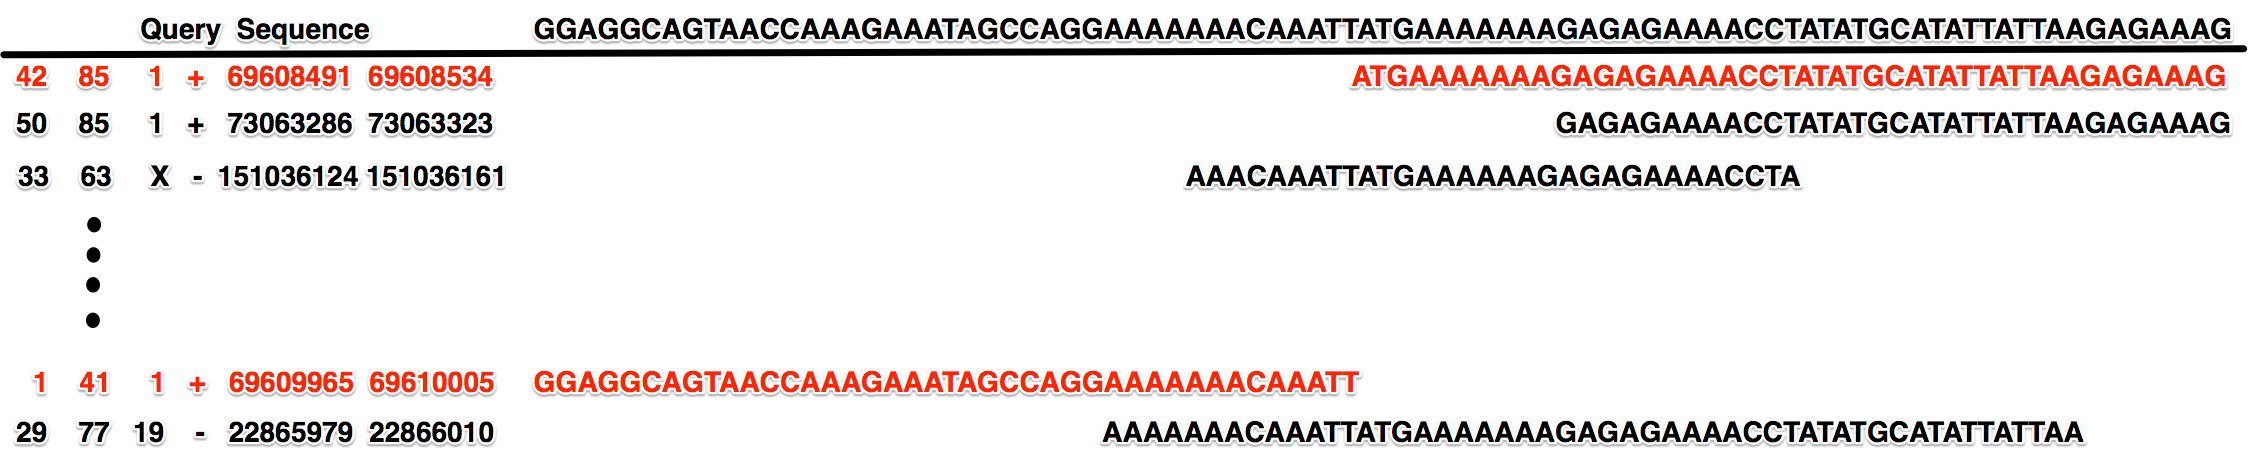
\includegraphics[scale = 0.46]{motivation/motivation2.png}
\captionof{figure}{The alignments to the reference are shown to the left, and
the alignments in red show the optimal cover for the query.}
\vspace{10mm}

We examine $m$ initial alignments of the query $Q$ of length $n$ against a
target genome $T$ using an aligner e.g. LASTZ \cite{rsharris} that can find all 
alignments that score above a pre-determined threshold. These alignments are
input to a modified Smith-Waterman algorithm, which then determines the optimal
coverage set for the query from among the alignments. A variant with constant 
jump penalty requires $O(mn)$  time to calculate the optimal alignment score, 
whereas the variant with variable jump weights requires $O(m^2n)$ time. 
$O(mn)$ space is required to store the  scoring matrix represented by $V$, 
as well as a trace-back matrix $T$ which can  then be used to recover the 
alignments for the best coverage set. 

\section*{Simulations}

\vspace{10mm}
{
\centering
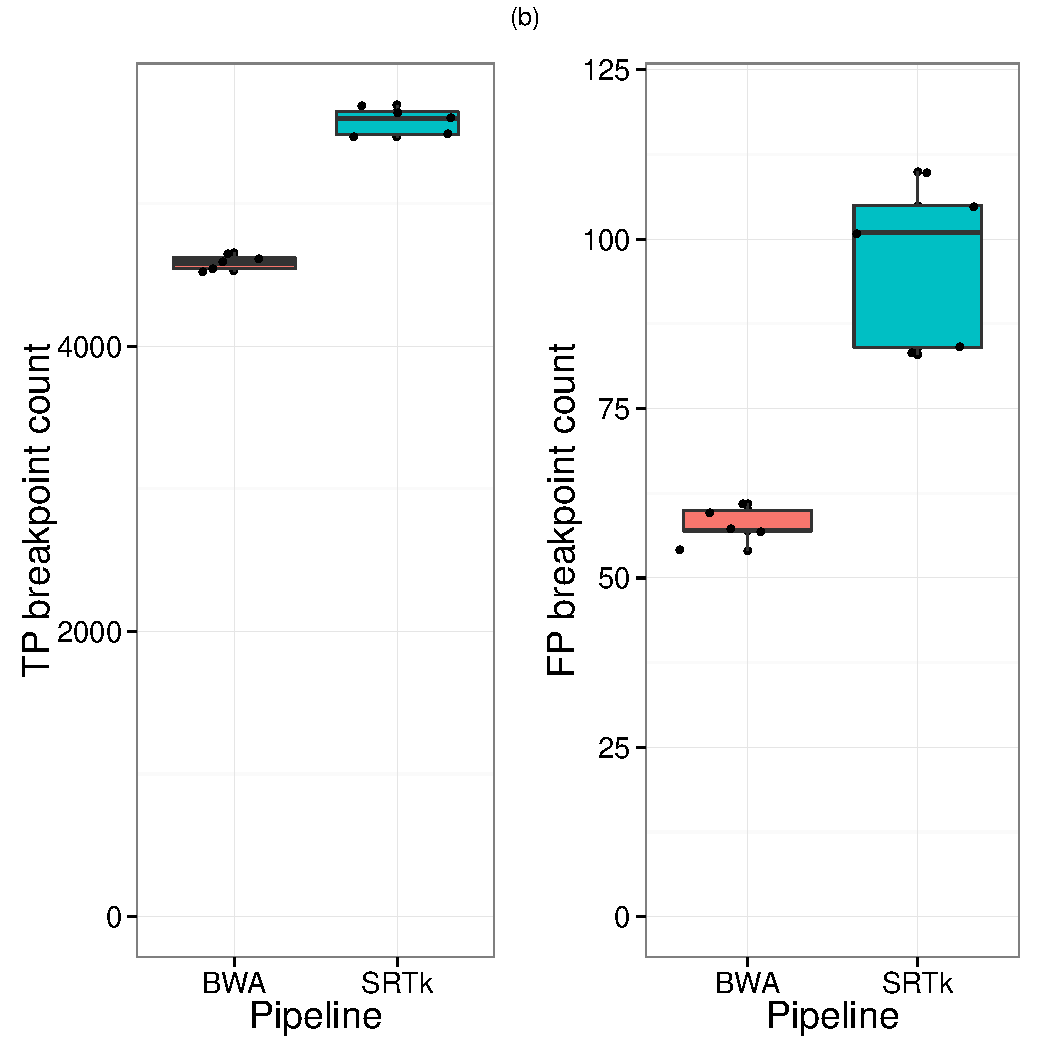
\includegraphics[scale = 0.8]{illumina_sim/repeats.pdf}
\hspace{25mm}
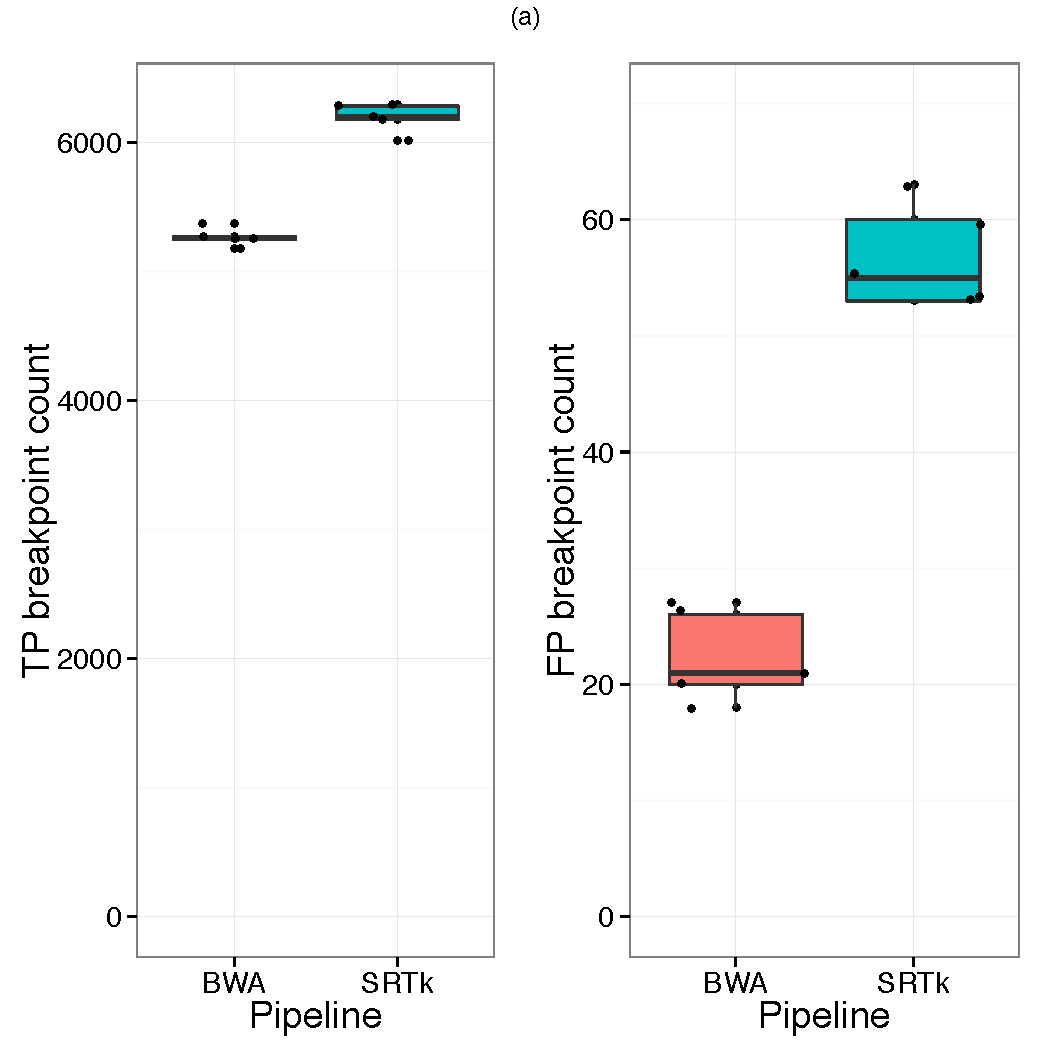
\includegraphics[scale = 0.8]{illumina_sim/random.pdf} 
\vspace{-3mm}
\captionof{figure}{Performance of SRTk+LUMPY compared to BWA+LUMPY when (a)
random breakpoints on hg19 are simulated, (b) breakpoints with bias towards
repeats on hg19 are simulated.}
}
\vspace{10mm}

We simulated 10,000 SVs (equal number of deletions, insertions, inversions and
duplications, with size distributions inferred from the results of the 1000
genomes project) with breakpoints that were placed (a) uniformly across the human
genome and (b) with a bias towards repeats
in the human  genome using RSVsim \cite{Bartenhagen01072013}.  We ran SRTk and the output was
supplied to LUMPY \cite{ryan} to call the variants. We show the count of
true-positive and the false-positive exact breakpoints that were identified as the simulations were repeated 5 times.

%%%Column 3
\section*{Prostate Cancer Genome Sequencing Project}

37 tumor-normal pairs sequenced as part of the Prostate Cancer
Genome Sequencing Project
\url{http://www.ncbi.nlm.nih.gov/projects/gap/cgi-bin/study.cgi?study_id=phs000447.v1.p1}
analyzed for breakpoints using SRTk+LUMPY.

{
\centering
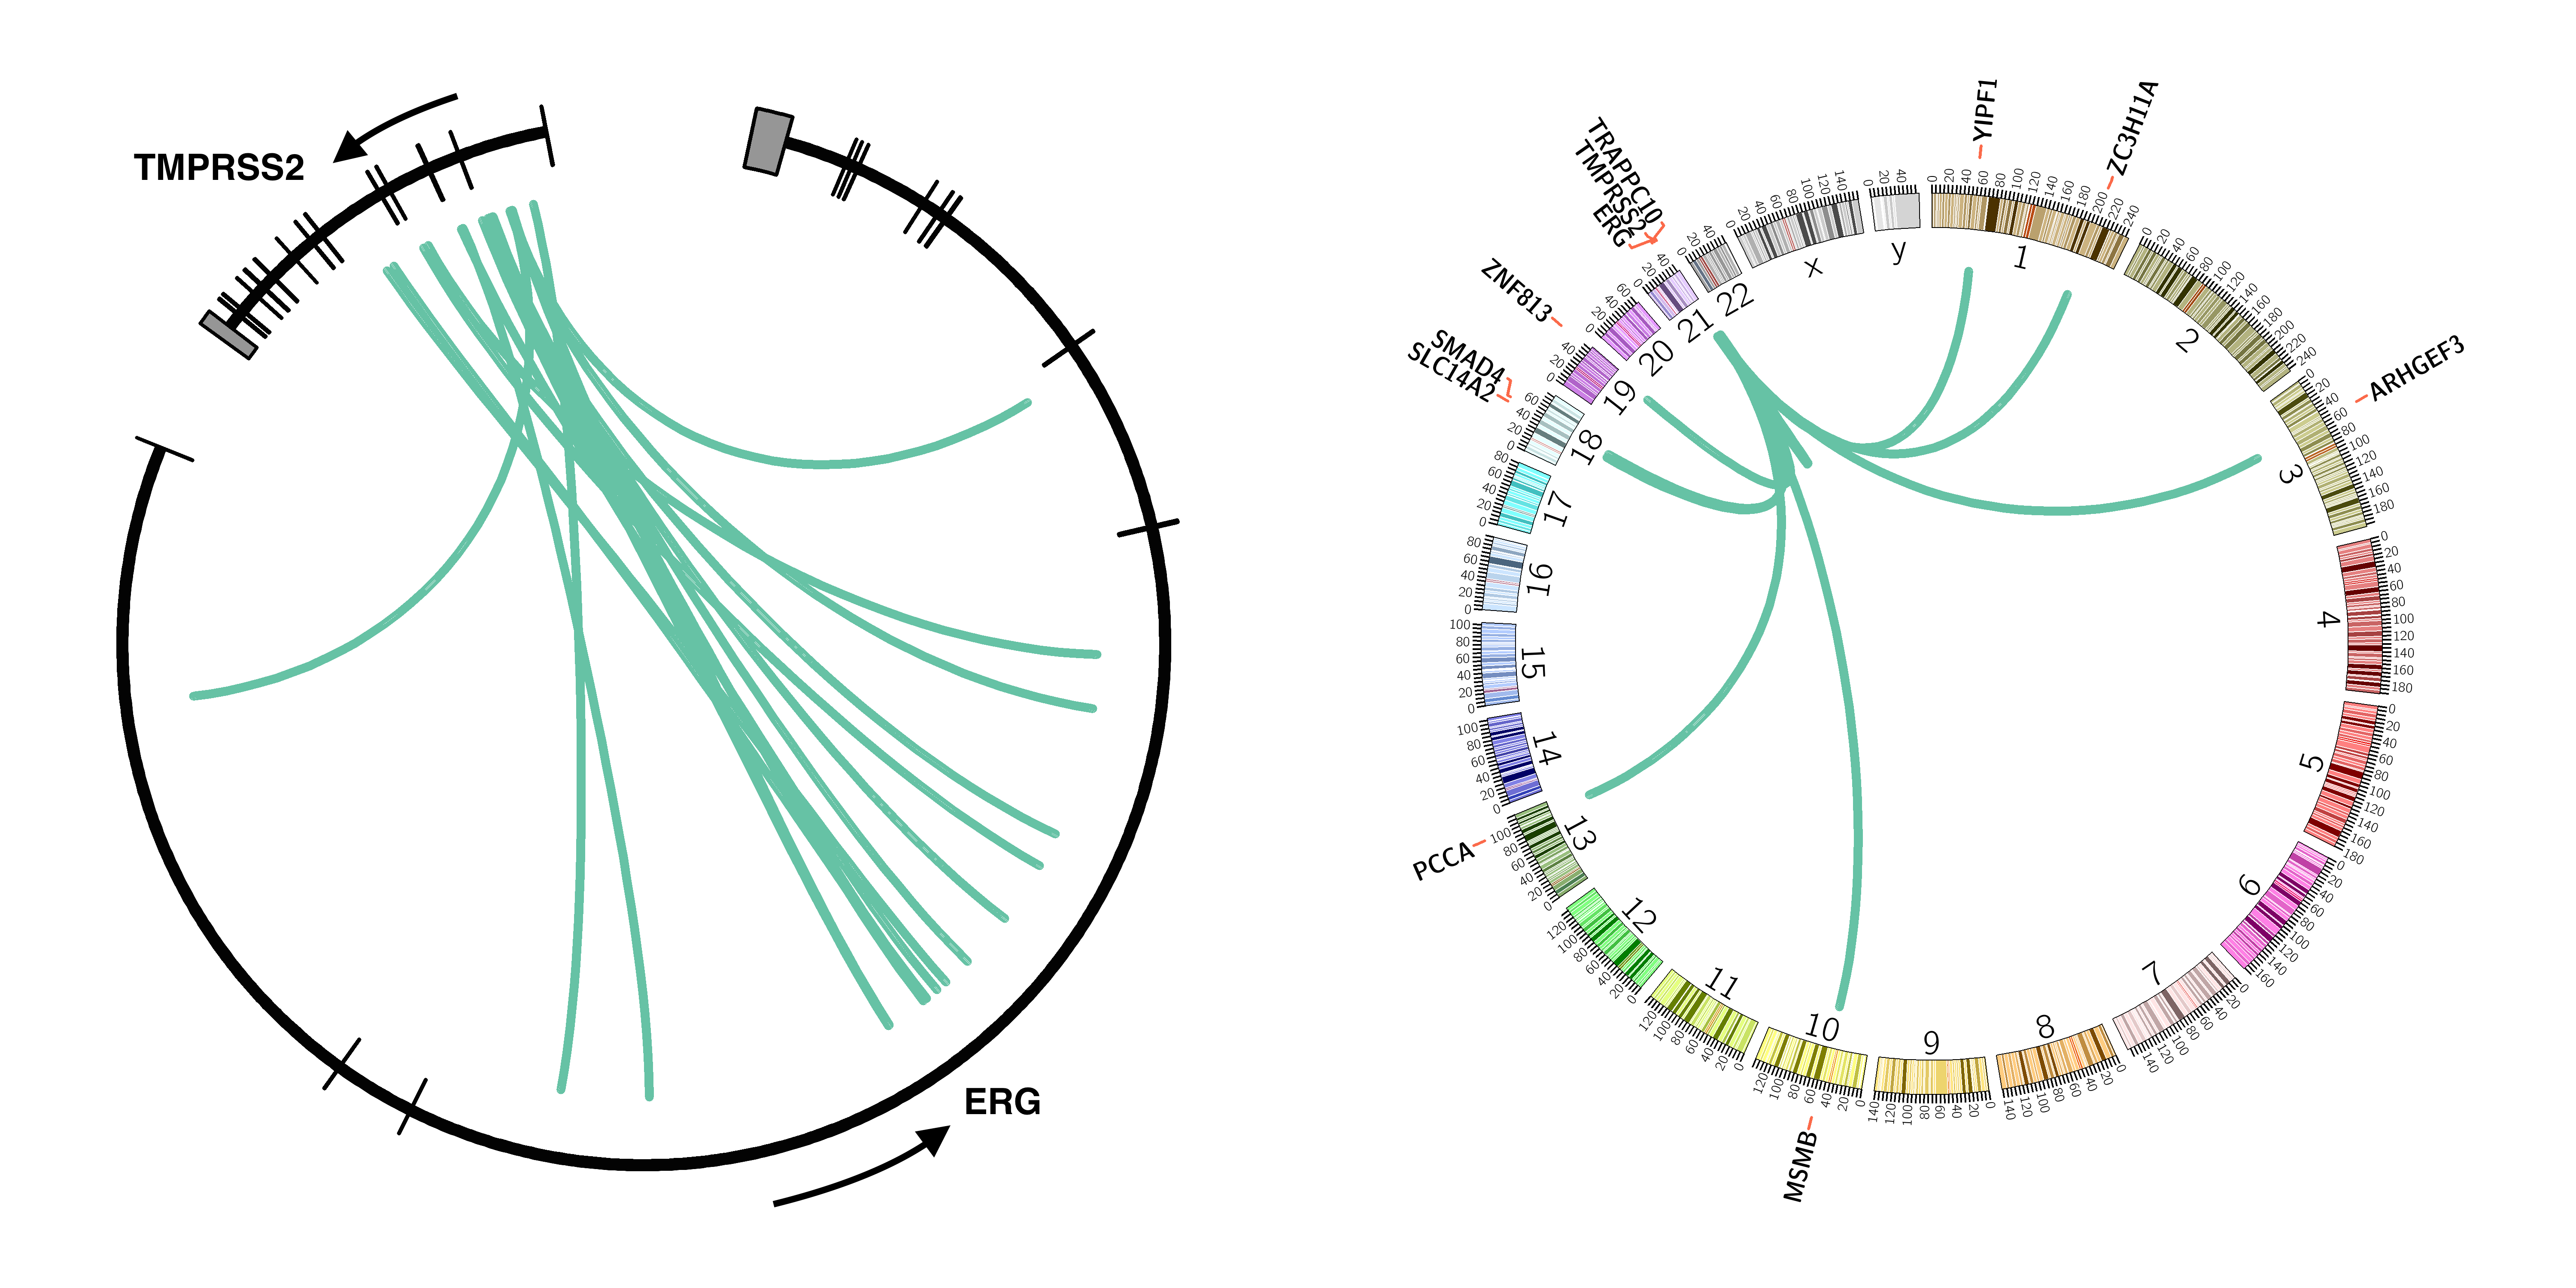
\includegraphics[scale = 0.25]{circos.png} 
\captionof{figure}{Location of breakpoints in TMPRSS2 and ERG found in 13 of the
tumor samples. Also shown are the other genes that share breakpoints with
TMPRSS2 in at least one of the samples.}
}
\vspace{15mm}
{
\centering
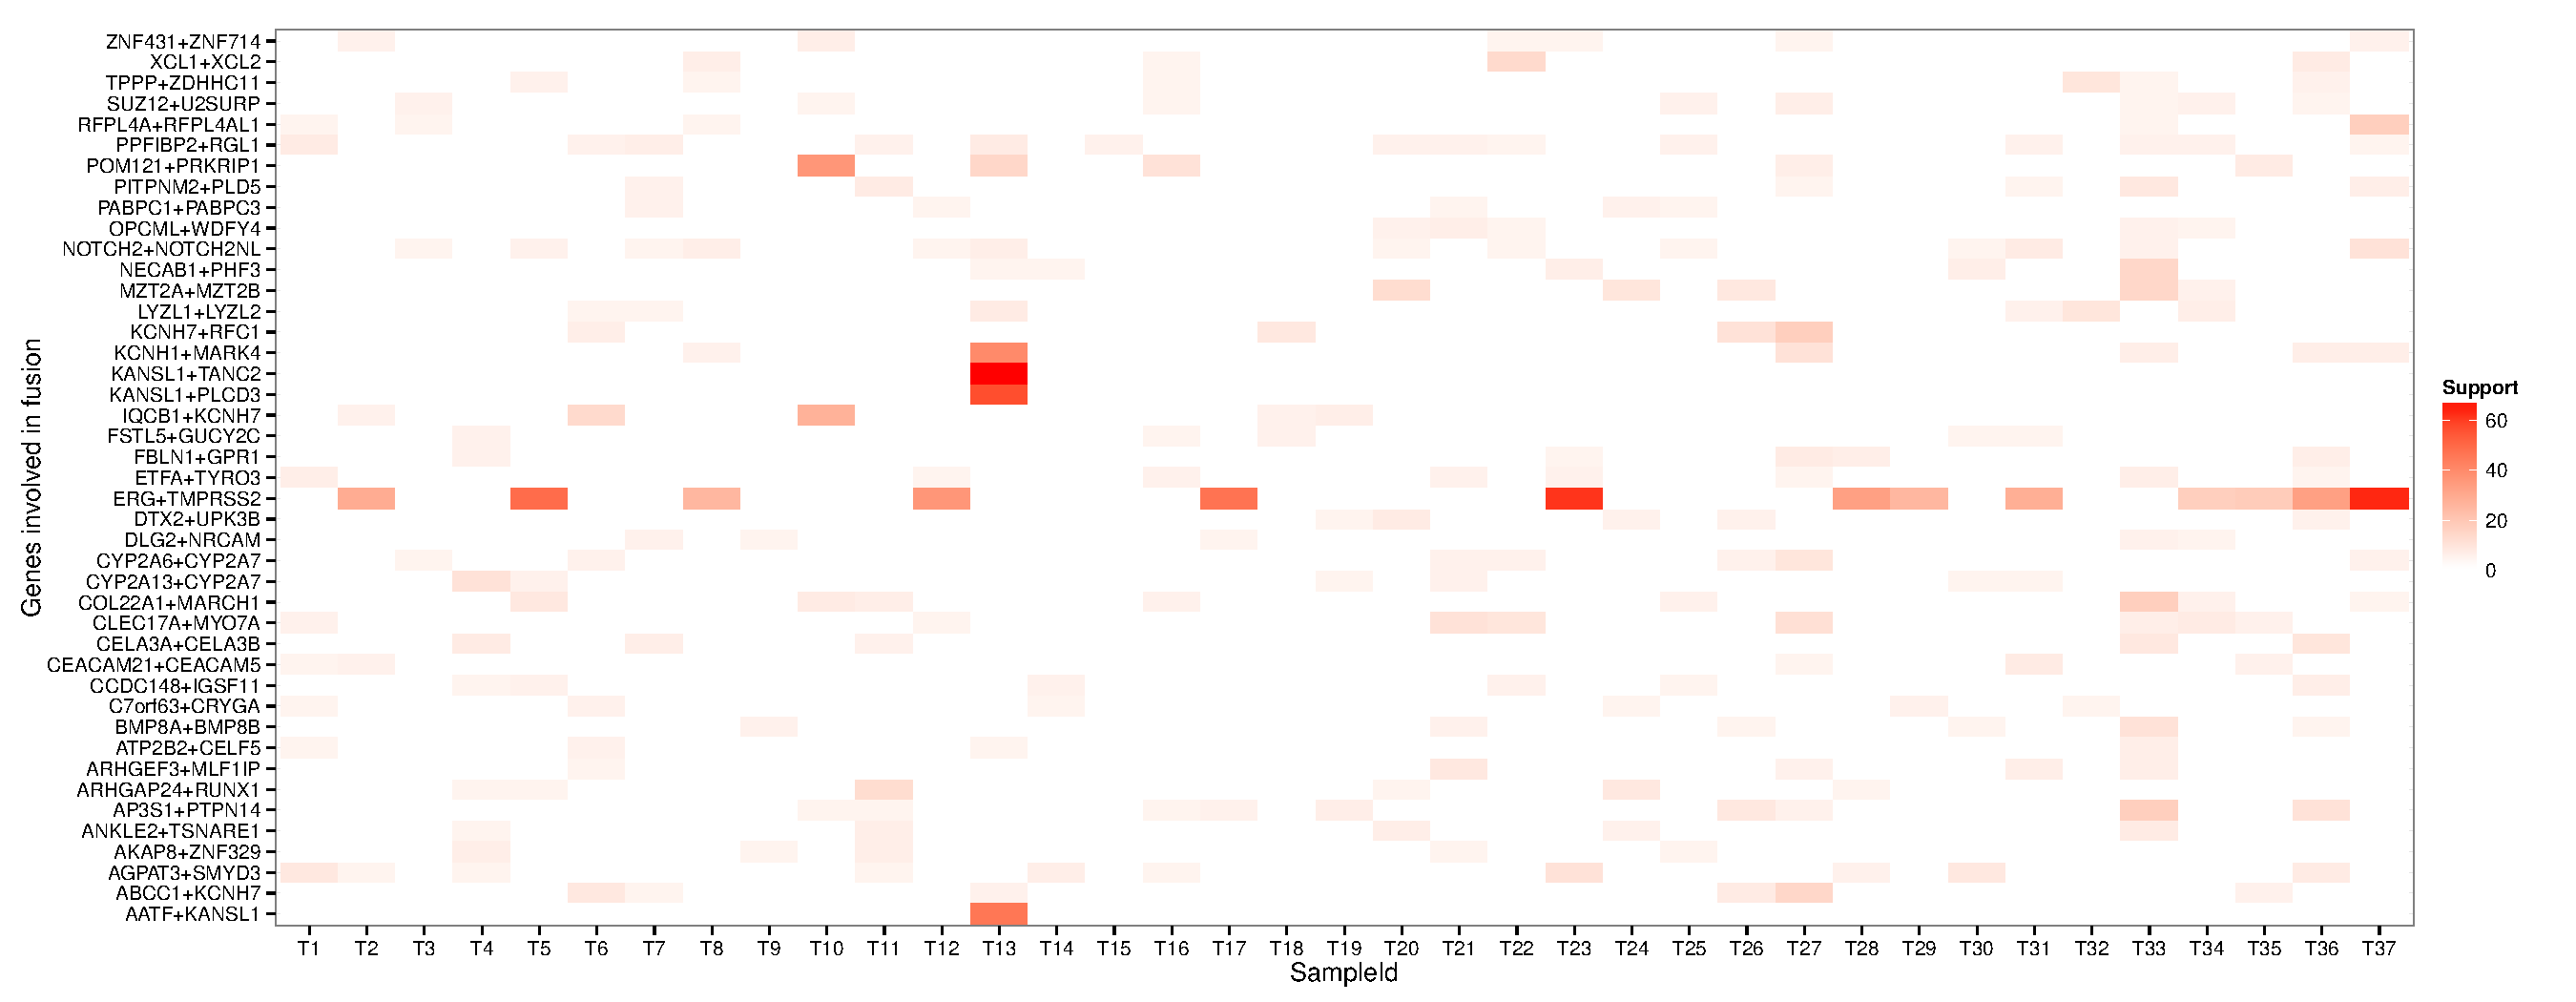
\includegraphics[scale = 1.0]{putative_fusion_heatmap/tumor.pdf}
\captionof{figure}{Putative gene fusions in the 37 tumor samples. Only the
location of the breakpoint and direction of transcription were considered in
making these predictions}
}
\vspace{15mm}
{
\centering
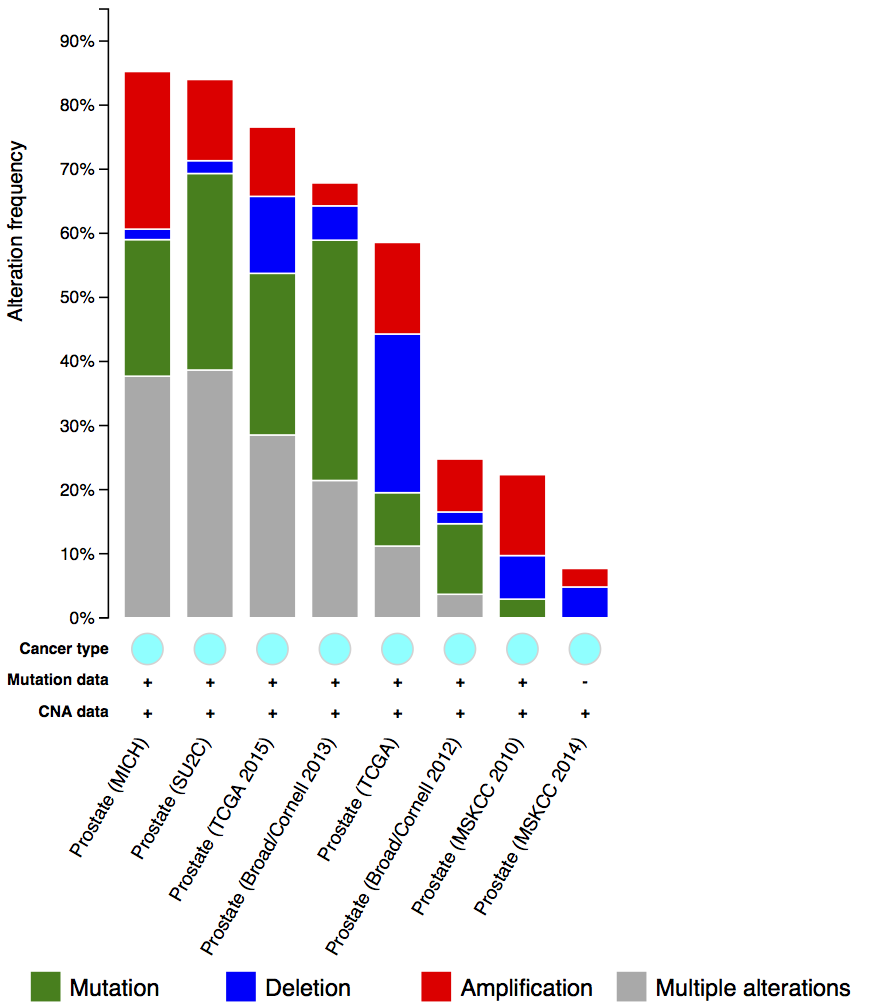
\includegraphics[scale = 1.5]{cbio.png}
\captionof{figure}{Identified genes play a significant role in the etiology of
Prostate Cancer. Shown here are the alterations reported in these genes by other
Prostate Cancer studies.}
}
\vspace{15mm}
{
\centering
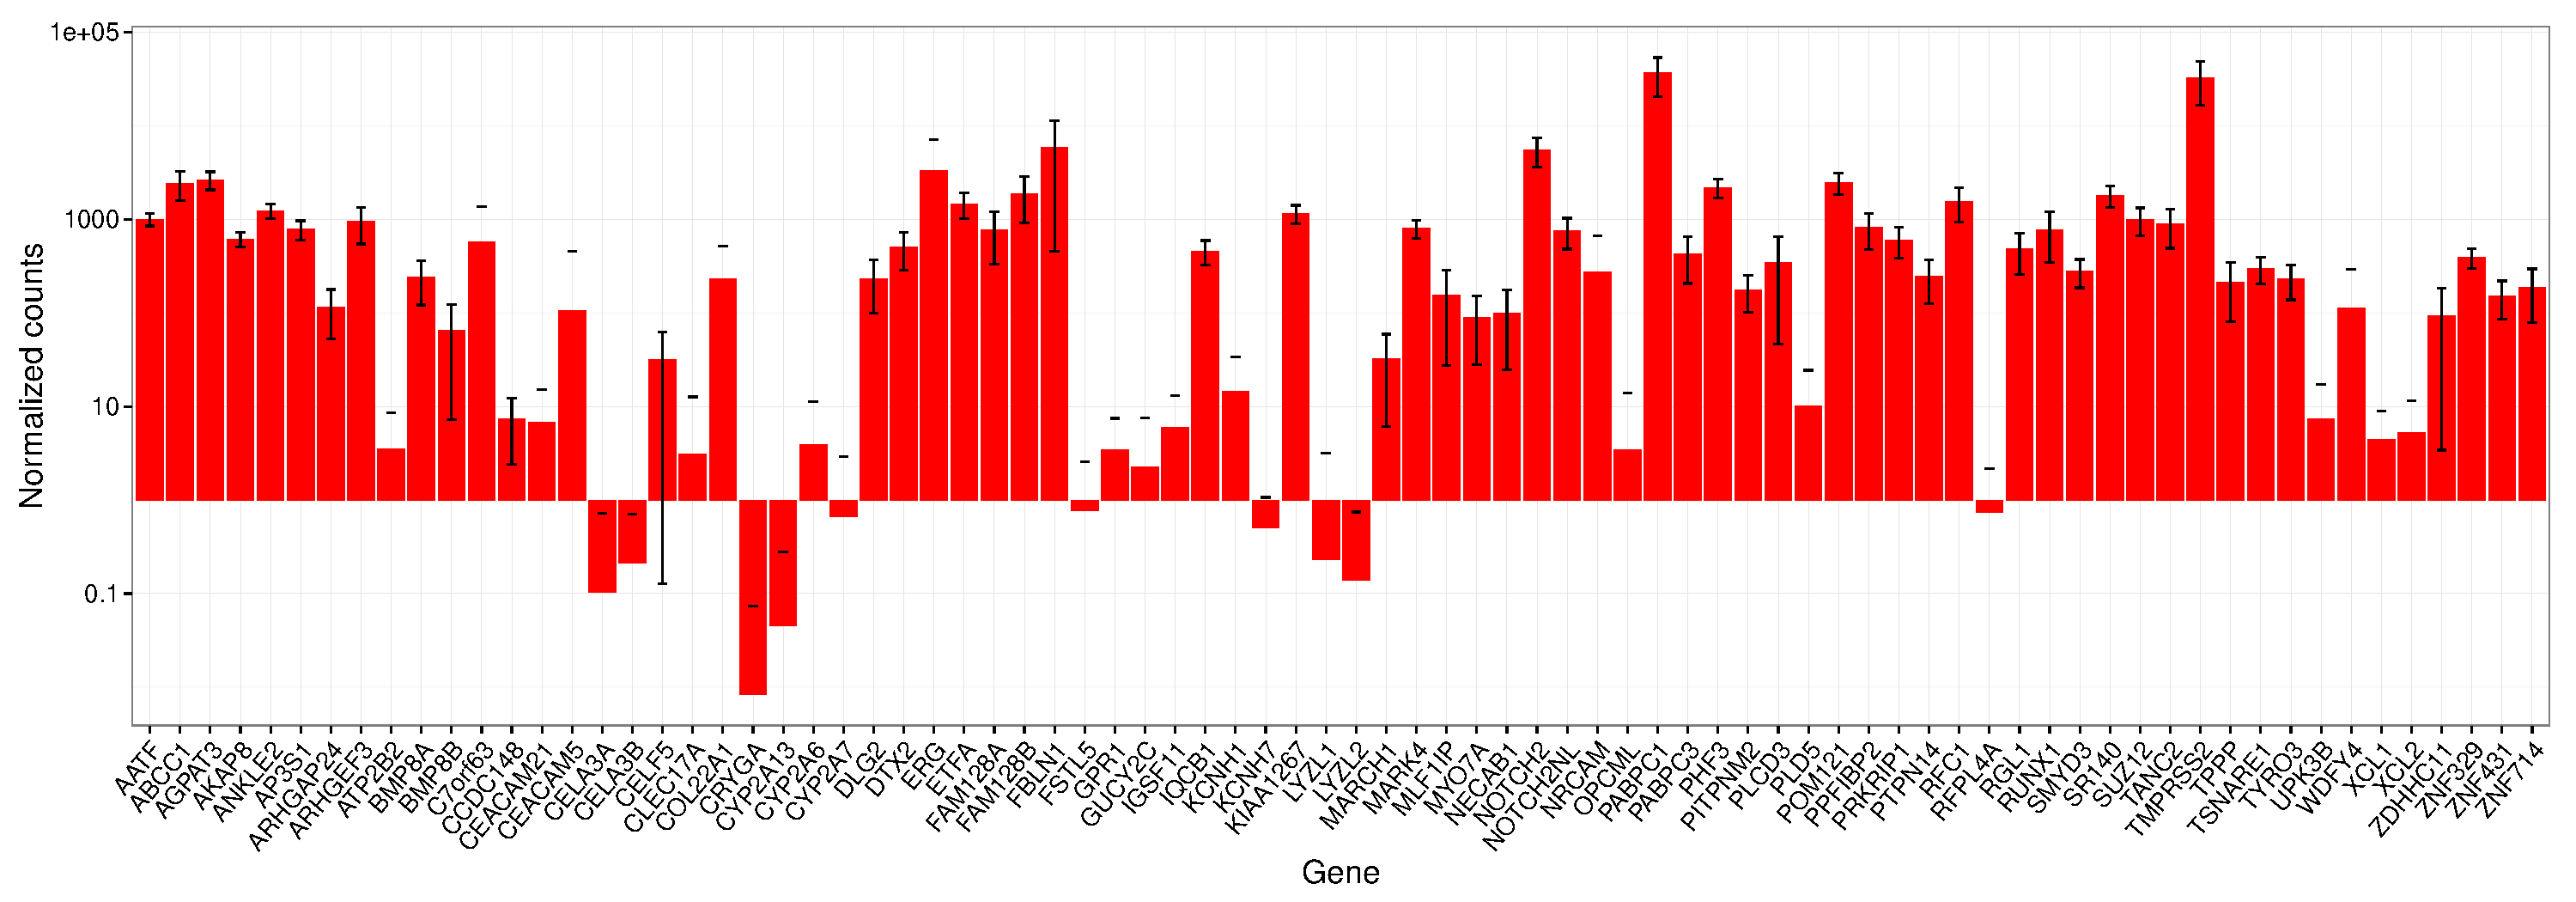
\includegraphics[scale = 0.75]{rnaseq/expression.pdf}
\captionof{figure}{Normalized read counts for the 81 genes in 178 tumor samples
that are included in the TCGA RNA-Seq dataset. Many of the candidate genes are
expressed in the tumor samples.}
}

\printbibliography

\end{multicols}
\end{document}
